\documentclass{article}
\usepackage[utf8]{inputenc}
\usepackage{graphicx}
\setlength{\parindent}{0pt}
\usepackage[left=3cm, right=3cm, top=3cm, bottom=3cm]{geometry}

\title{LabMuoni}
\author{giulia lavizzari}
\date{November 2021}

\begin{document}

\maketitle

\section{12/11/21}
Primo approcio alla strumentazione. Sembrava ancora che le cose funzionassero :)

\section{17/11/21}
Caratterizzazione dei moduli
\\\\\textbf{Discriminator threshold settings:}
\begin{itemize}
    \item range threshold
    \item corrispondenza tra valore della soglia e altezza dell'impulso
\end{itemize}\
\textbf{Timer counter settings:}
\begin{itemize}
    \item lo stesso numero di conteggi viene osservato con tutti i canali (impulsatore $\rightarrow$ discriminatore con soglia bassa $\rightarrow$ counter)
\end{itemize}


\section{19/11/21}
\textbf{Caratterizzazione dei moduli con impulsatore (onde quadre) e caratterizzazione risposta scintillatore con scelta della soglia}\\\\
Carattatterizzazione nuovo discriminatore: range soglia per ogni canale, risposta corretta del modulo all'onda quadra.\\\\
Scelta della soglia: discriminatore + scintillatore zero. Plot rate vs thr, si cerca il plateau. HV = 900V, t=100s
\begin{figure}
    \centering
    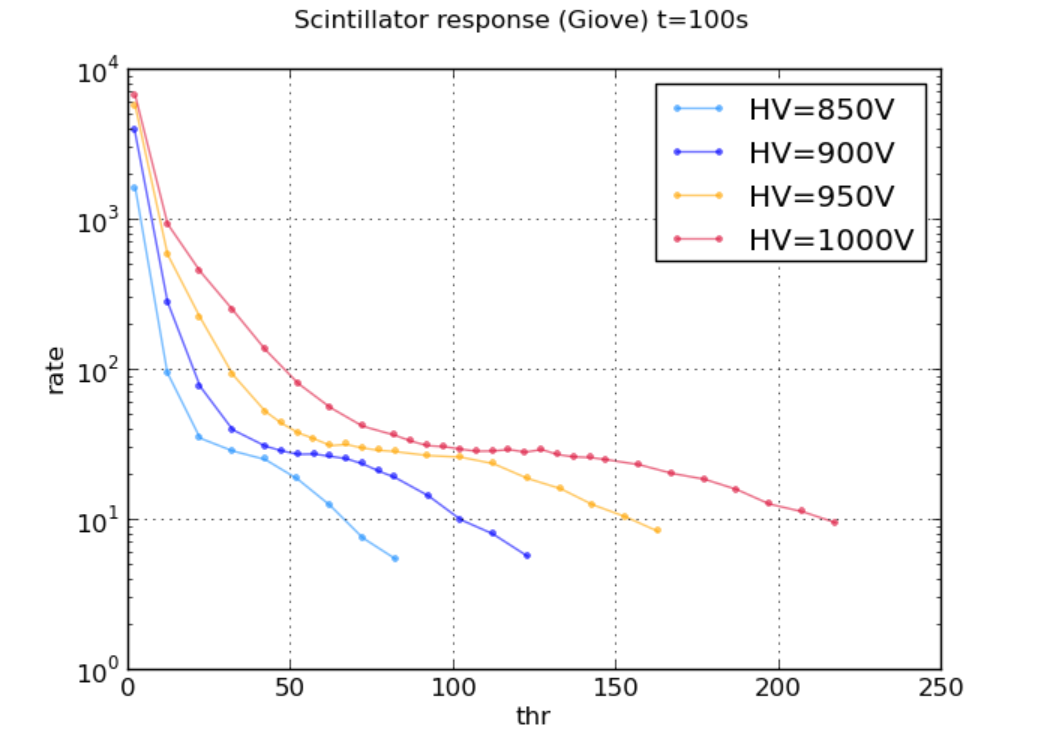
\includegraphics[width=0.9\textwidth]{dati1.PNG}
\end{figure}



\section{24/11/21}
\textbf{scelti i nomiii}
Giove (G1)
Giunone (G2)
Minerva (M)\\\\
\textbf{caratterizzazione risposta scintillatore al variare della soglia}\\
Caratterizzazione della risposta di ciascuno dei tre scintillatori.\\\\
Tip per il futuro: valutare la tensione di bias di Minerva in base alle efficienze: siccome per Minerva non si vede bene il plateau, è difficile scegliere la soglia e bias. Ci si mette in una situa in cui G1 - M - G2 e con soglie di G1 e G2 tali da essere nel plateau (così per loro siamo sicuri di beccare i muoni). Se vedo una coinc per G1 e G2 ma non per M vuol dire che sto tagliando i muoni, quindi regolare thr e bias di M.\\\\
\textbf{giulia ha scoperto i colori ;)}
Siamo felici :D \\\\


\section{26/11/21}
Stiamo andanso avanti con la stessa cosa. Oggi siamo meno felici. Abbiamo però scoperto che il primo punto dei grafici (soglia bassissima, 2mV) ha un rate sovrastimato perchè al passaggio di un singolo impulso si aprono più finestre nel discriminatore. Questo già da 12mV non succede più (per Minerva abbiamo ampliato la finestra temporale affinchè non succedesse)\\\\
\textbf{Finestra temporale discr:} 65ns per G1,G2 (ch 1,3 discr) - 80s (ch 2 discr) per M

\section{01/12/21}
Caro diario,\\
Niente di nuovo sul fronte occidentale. Andiamo avanti con le misure. Speriamo di vedere qualche plateau per Minerva. Nessun plateau è stato trovato per Minerva. Ma vabbé.\\\\
Recuperiamo i moduli per fare le misure con le efficienze (non caratterizziamo i moduli, ci fidiamo perchè dobbiamo fare le misure prima di Natale)\\\\
Come stai psicologicamente? Male.



\section{03/12/21}
Oggi siamo carichi: cominciano le misure di coincidenze. Samu ha la tabella in cui è programmata l'unità logica.\\\\
LOGICA $\rightarrow$ SCALER:\\
la logica in modalità fall/rise dà output con rise time $\leq 2ns$  che va bene come input dello scaler (perchè prende input -800mV dando 1 come out, che è corretto perchè i NIM veloci sono tra -14 e -18 mA e -800mV cade proprio in mezzo, considerando la resistenza 50ohm)\\\\
Nella config per le coincidenze abbiamo mandato l'output del clock dello scaler nel fi/fo per avere 3 segnali da mandare ai 3 contatori che fanno le 3 coincidenze. Così facendo si introducono dei ritardi: 2ns + 3ns (cavi) + 7ns (fi/fo) quindi 12ns. Il rate di muoni è circa 40 Hz quindi tempo tra due muoni è 1/40 s = 0.025s $>>$ 12ns. Quindi non crediamo che la cosa dia problemi


\section{10/12/21}
MISURE DI COINCIDENZA\\
ritardi linee (scint - discr - logica):
\begin{itemize}
    \item G1 = 10 ns + 2ns
    \item G2 = 8 ns + 2 ns
    \item M = 5 ns + 2ns
\end{itemize}
Abbiamo concluso che sta cosa non ci crea problemi per le coincidenze perché tanto gli impulsi sono larghi 60-80ns [il resolving time è $\sim$ ns]
\\\\
FAST CHARACTERIZATION\\
Counter: ok\\
Fi/fo: ok\\
Logica: ok

\section{15/12/21}
\textbf{GIACHERO:}\\
lab/CAENSCOPE../bin $\rightarrow$ ./scope\\
Quando si apre: connect. Scegliere la finestra in mezzo uguale a 0, non 1\\\\

\textbf{TERRANOVA:}\\
Scan in tensione e non in soglie per fare l'efficienza (perchè la tensione varia in modo brusco, la soglia cambia meno la risposta).\\
In generale obv campionamento fine dove i cambi sono abrupt\\
\textbf{Tensione e soglia dei due scint esterni fissate}, centrale variabile\\
Come scegliere la tensione associata a ogni voltaggio? Ragionamento sulle ampiezze del segnale anodico: guardo un punto (V, thr) nel quale mi trovo bene e vedo a che altezza percentuale dell'ampiezza media della waveform sono. Fisso tale percentuale e ogni volta che cambio tensione cambio di conseguenza l'altezza della soglia, in modo da avere la stessa percentuale fissata. La chiave è che 
\textbf{la waveform media è dominata dai Muoni!!} 
ragion per cui il ragionamento sul rapporto dei rate non funzionava (perchè a denom c'è il numero di imusi a soglia zero: questo contiene i segnali bassi, aka rumore, quindi non è tarato sui mu ma sballa).\\\\
nostre scelte di conseguenza:
\begin{itemize}
    \item Scegliamo la percentuale prendendo come punto di riferimento un punto a metà plateau di uno dei due scintillatori belli. Questa percent poi si applicherà a tutto il resto (alternativa: scegliere percentuale per pulire dallo schifo il segnale di M: temiamo che così il rate sarebbe troppo basso quindi non lo facciamo)
    \item Come scegliamo le tensioni di quelli esterni? Sulla base delle relazioni degli altri... un punto di partenza dobbiamo pur prenderlo (tensioni almeno tali da vedere un pateau nei rate di singola)
\end{itemize}


\section{17/12}
Change of plans: possiamo trovare il Working Point ottimale anche per Minerva! Grafico del rate di singola e tripla per minerva. Quello di tripla, dominato nettamente dai muoni e non dall'ambientale, è costante finchè non raggiungiamo un valore di soglia a cui iniziamo a tagliare i muoni. Il WP ottimale è quindi subito prima del calo. Oggi cerchiamo questo, a quel punto faremo uno scan in tensioni e soglie per trovare i valori ottimali (mappa 2D con colori)\\\\
Faremo scan con intervalli di thr circa fittati (rette)

\section{22/12/21}
Abbiamo fatto il lavoro detto al punto prima (sta in effSingle, quello solo per minerva. Abbiamo dovuto rifare le eff rispetto a quelle cje avevamo già perchè i conteggi di singola erano di G1 o G2).\\\\
primi Valori di efficienza per M: up to 0.99! Questo sta in effMultiple\\\\
\textbf{link di Giachero per guida su git https://rogerdudler.github.io/git-guide/}\\\\
git add "filename"\\
git add * (per le repo non metto asterisco)\\
git commit -m "my commit"\\
git push https://github.com/GiuliaLavizzari/LabMuoni main\\
SEMPRE FARE git pull PRIMA DI QUALSIASI PUSH E MAI CANCELLARE COSE IN LOCALE\\


\end{document}